\section{Exploratory Data Analysis}
\label{chap:eda}

Exploratory data analysis uses statistical metrics to gain an understanding of the raw data.
In this work, exploratory data analysis also includes data partitioning for training, validation, and testing machine learning models and trading strategies, eliminating data drift, adding additional features, as well as scaling and dimension reduction.

It should be noted that apart from the data splitting, which is a general step in the process, the following steps are only relevant for the machine learning models and not for the classic trading strategies introduced later.

\subsection{Dividing the Data}

Unlike classic machine learning processes, where data is split into three subsets, named train-, validation-, and test-set, here the data is split in four subsets.
The fourth dataset is used for backtesting the real trading strategy, and is therefore not part of the machine learning process but plays an important role in developing the final trading strategy.
In contrast, the test-set is only part of the machine learning process and is not used for evaluating or backtesting trading strategies.
This distinction was made so that the critical phases (testing machine learning models and testing trading strategies) cannot influence each other.

\begin{table}[H]
    \centering
    \begin{tabular}{ L{1.5cm} >{\centering\arraybackslash}m{4cm} >{\centering\arraybackslash}m{2cm} P{2.5cm} P{1.5cm} }
        \toprule
        \textbf{Set} & From & To & No.
        of Datapoints & \% of All Data
        \\
        \midrule
        \textbf{Complete} & \makecell{08/05/2022 \\ 10:00 UTC+2} & \makecell{06/17/2025 \\ 11:30 UTC+2} & $1,507,598$ & \\
        \addlinespace[0.2em]
        \textbf{Train} & \makecell{08/05/2022 \\ 10:00 UTC+2} & \makecell{04/30/2024 \\ 23:59 UTC+2} & $913,684$ & $60.6\%$ \\
        \addlinespace[0.2em]
        \textbf{Validation} & \makecell{05/01/2024 \\ 00:00 UTC+2} & \makecell{09/30/2024 \\ 23:59 UTC+2} & $220,320$ & $14.6\%$ \\
        \addlinespace[0.2em]
        \textbf{Test} & \makecell{10/01/2024 \\ 00:00 UTC+2} & \makecell{12/31/2024 \\ 23:59 UTC+2} & $132,482$ & $8.8\%$ \\
        \addlinespace[0.2em]
        \textbf{Backtest} & \makecell{01/01/2025 \\ 00:00 UTC+2} & \makecell{06/17/2025 \\ 11:30 UTC+2} & $241,111$ & $15.9\%$ \\
        \addlinespace[0.2em]
        \bottomrule
    \end{tabular}
    \caption{Data Split}
    \label{tbl:data-split}
\end{table}

\noindent
After the splitting, the four subsets have the following summaries:

\begin{table}[H]
    \centering
    \begin{tabular}{L{1.5cm}ccccc}
        \toprule
        & Open & High & Low & Close & Volume
        \\
        \midrule
        & Open & High & Low & Close & Volume
        \\
        \textbf{count} & 913,684.0 & 913,684.0 & 913,684.0 & 913,684.0 & 913,684.0 \\
        \textbf{mean}  & 1,933.4   & 1,933.95  & 1,932.85  & 1,933.4   & 7.58      \\
        \textbf{std}   & 619.6    & 619.92   & 619.28   & 619.6    & 105.09   \\
        \textbf{min}   & 1,074.35  & 1,077.45  & 1,064.05  & 1,074.35  & 0.0       \\
        \textbf{25\%}  & 1,578.44  & 1,578.89  & 1,577.99  & 1,578.44  & 0.0       \\
        \textbf{50\%}  & 1,801.52  & 1,801.81  & 1,801.13  & 1,801.52  & 0.05      \\
        \textbf{75\%}  & 2,083.4   & 2,083.84  & 2,083.05  & 2,083.4   & 2.02      \\
        \textbf{max}   & 4,098.5   & 4,099.48  & 4,096.35  & 4,098.5   & 31,350.65 \\
        \bottomrule
    \end{tabular}
    \caption{Train Data}
    \label{tbl:train-data}
\end{table}

\begin{table}[H]
    \centering
    \begin{tabular}{L{1.5cm}ccccc}
        \toprule
        & Open & High & Low & Close & Volume
        \\
        \midrule
        \textbf{count} & 220,320.0 & 220,320.0 & 220,320.0 & 220,320.0 & 220,320.0 \\
        \textbf{mean}  & 3,050.36  & 3,051.3   & 3,049.4   & 3,050.36  & 2.89      \\
        \textbf{std}   & 473.4    & 473.45   & 473.34   & 473.4    & 21.45    \\
        \textbf{min}   & 2,111.8   & 2,160.4   & 2,088.13  & 2,111.8   & 0.0       \\
        \textbf{25\%}  & 2,617.31  & 2,618.04  & 2,616.71  & 2,617.31  & 0.0       \\
        \textbf{50\%}  & 3,063.4   & 3,064.31  & 3,062.43  & 3,063.4   & 0.12      \\
        \textbf{75\%}  & 3,462.22  & 3,463.29  & 3,461.21  & 3,462.22  & 1.32      \\
        \textbf{max}   & 3,974.68  & 3,976.96  & 3,969.94  & 3,974.68  & 4,972.18  \\
        \bottomrule
    \end{tabular}
    \caption{Validation Data}
    \label{tbl:validation-data}
\end{table}

\begin{table}[H]
    \centering
    \begin{tabular}{L{1.5cm}ccccc}
        \toprule
        & Open & High & Low & Close & Volume
        \\
        \midrule
        \textbf{count} & 132,482.0 & 132,482.0 & 132,482.0 & 132,482.0 & 132,482.0 \\
        \textbf{mean}  & 3,093.93  & 3,095.27  & 3,092.58  & 3,093.94  & 4.42      \\
        \textbf{std}   & 531.85   & 532.29   & 531.4    & 531.85   & 18.42    \\
        \textbf{min}   & 2,309.01  & 2,311.73  & 2,307.73  & 2,309.01  & 0.0       \\
        \textbf{25\%}  & 2,541.8   & 2,542.65  & 2,540.94  & 2,541.8   & 0.08      \\
        \textbf{50\%}  & 3,143.69  & 3,145.38  & 3,142.02  & 3,143.7   & 0.68      \\
        \textbf{75\%}  & 3,487.9   & 3,489.46  & 3,486.33  & 3,487.9   & 2.92      \\
        \textbf{max}   & 4,107.28  & 4,112.68  & 4,102.6   & 4,107.28  & 1,341.05  \\
        \bottomrule
    \end{tabular}
    \caption{Test Data}
    \label{tbl:test-data}
\end{table}

\begin{table}[H]
    \centering
    \begin{tabular}{L{1.5cm}ccccc}
        \toprule
        & Open & High & Low & Close & Volume
        \\
        \midrule
        \textbf{count} & 241,111.0 & 241,111.0 & 241,111.0 & 241,111.0 & 241,111.0 \\
        \textbf{mean}  & 2,432.57  & 2,433.77  & 2,431.35  & 2,432.57  & 7.0       \\
        \textbf{std}   & 574.72   & 574.95   & 574.49   & 574.72   & 32.11    \\
        \textbf{min}   & 1,386.6   & 1,395.8   & 1,382.99  & 1,386.6   & 0.0       \\
        \textbf{25\%}  & 1,887.22  & 1,888.28  & 1,886.1   & 1,887.22  & 0.18      \\
        \textbf{50\%}  & 2,510.29  & 2,511.4   & 2,509.1   & 2,510.29  & 1.26      \\
        \textbf{75\%}  & 2,732.0   & 2,733.21  & 2,730.7   & 2,732.0   & 4.94      \\
        \textbf{max}   & 3,742.33  & 3,745.13  & 3,739.65  & 3,742.33  & 2,534.66  \\
        \bottomrule
    \end{tabular}
    \caption{Backtest Data}
    \label{tbl:backtest-data}
\end{table}

\subsection{Using Log-Returns}
\label{chap:log-returns}

In the summary statistics of the subsets (\autoref{tbl:train-data}, \autoref{tbl:validation-data}, \autoref{tbl:test-data}, \autoref{tbl:backtest-data}), it is noticeable that the mean values change over time.
This also becomes clear when visualizing the data (\autoref{fig:eth-data}).

\begin{figure}[H]
    \centering
    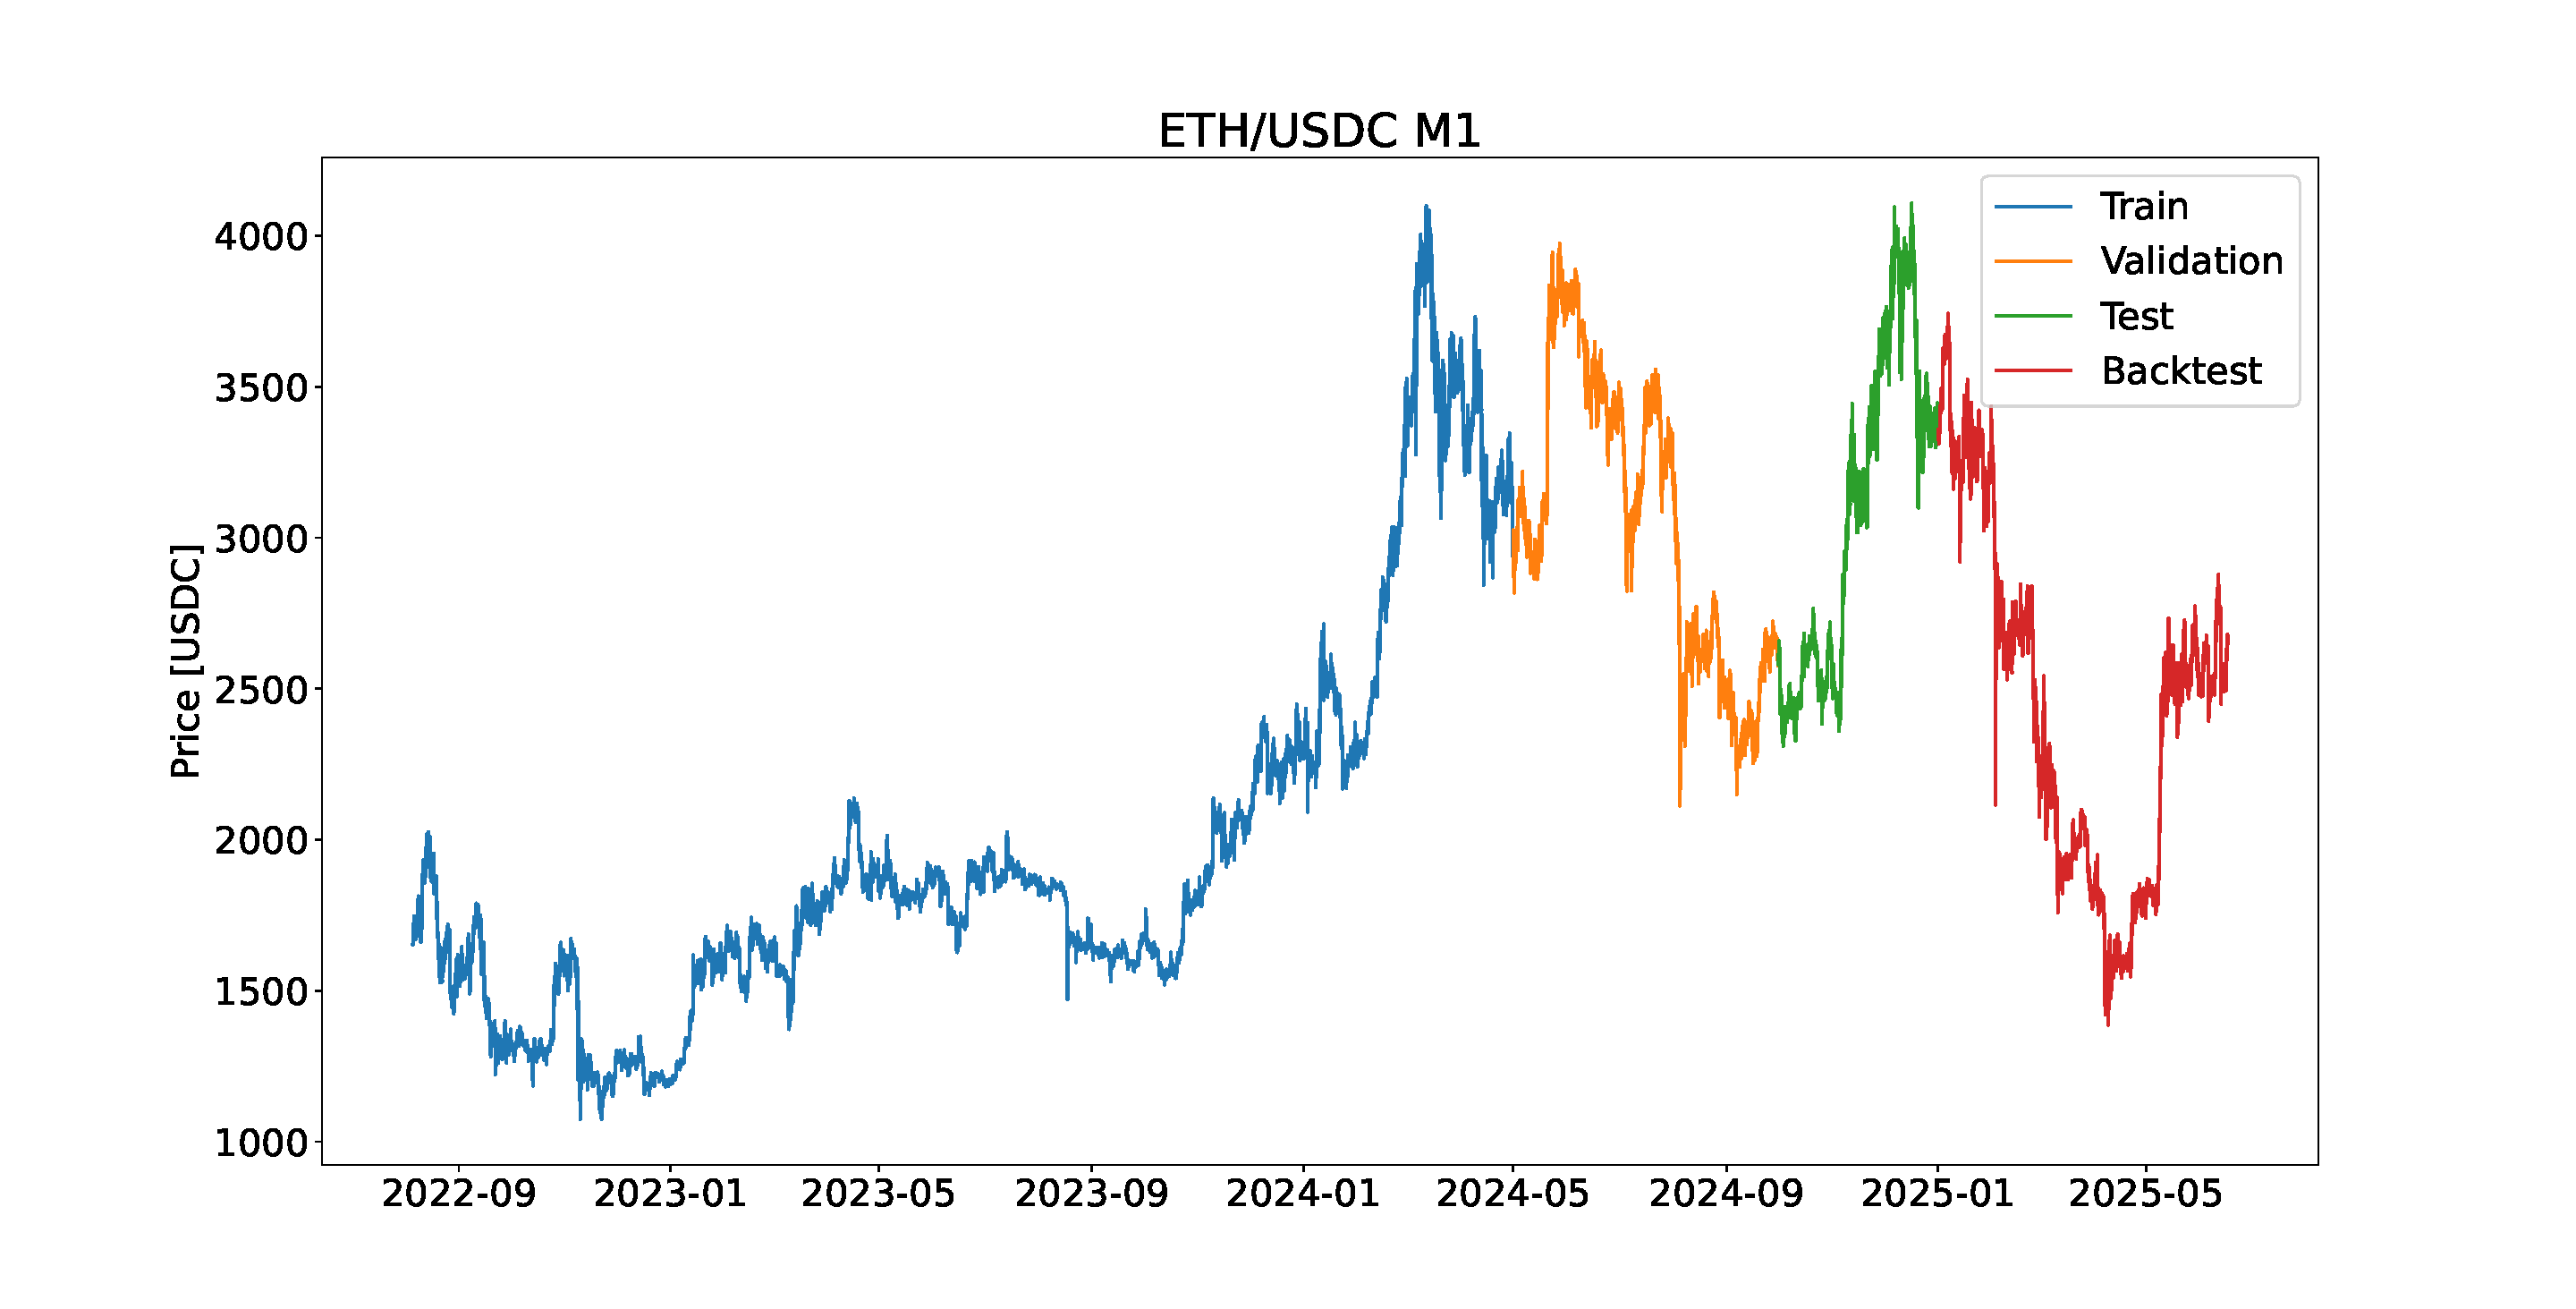
\includegraphics[width=\textwidth]{images/eda/ethusdc_price}
    \caption{Price Fluctuation of ETH in USDC}
    \label{fig:eth-data}
\end{figure}

\noindent
To avoid this data drift, the price is transformed to its logarithmic returns (also called log-returns).
These are calculated as follows \cite{log-returns}:

\[
    LogReturn_t = \ln\left(\frac{Price_t}{Price_{t-1}}\right)
\]

\noindent
After the transformation, the means and standard deviations in the subsets are very similar, and the data no longer drifts over time.
\autoref{tbl:stat-log-returns} shows the means and standard deviations after the logarithmic return transformation.
This was also confirmed by an augmented Dickey-Fuller test (ADF test).
The ADF test is a common statistical procedure for investigating whether a time series contains a unit root, which would indicate non-stationarity \cite{adf}.
In this context, the null hypothesis that the time series is non-stationary, i.e., exhibits a stochastic trend, was tested.
The test result yielded a p-value of 0.0, which is below the 5\% significance level, so the null hypothesis could be rejected.
This indicates that the time series is stationary and that there is no significant data drift over the period under consideration.
Additionally, \autoref{fig:eth-log-data} shows visually that the data drift is eliminated.

\begin{table}[H]
    \centering
    \begin{tabular}{L{3cm}cc}
        \toprule
        \textbf{Data Set}   & Mean    & Standard Deviation \\
        \midrule
        \textbf{Train}      & 6.5E-7  & 8.7E-4             \\
        \textbf{Validation} & -6.1E-7 & 9.4E-4             \\
        \textbf{Test}       & 1.8E-6  & 9.4E-4             \\
        \textbf{Backtest}   & -9.5E-7 & 1.1E-3             \\
        \bottomrule
    \end{tabular}
    \caption{Statistics after Logarithmic Returns Transformation}
    \label{tbl:stat-log-returns}
\end{table}

\begin{figure}[H]
    \centering
    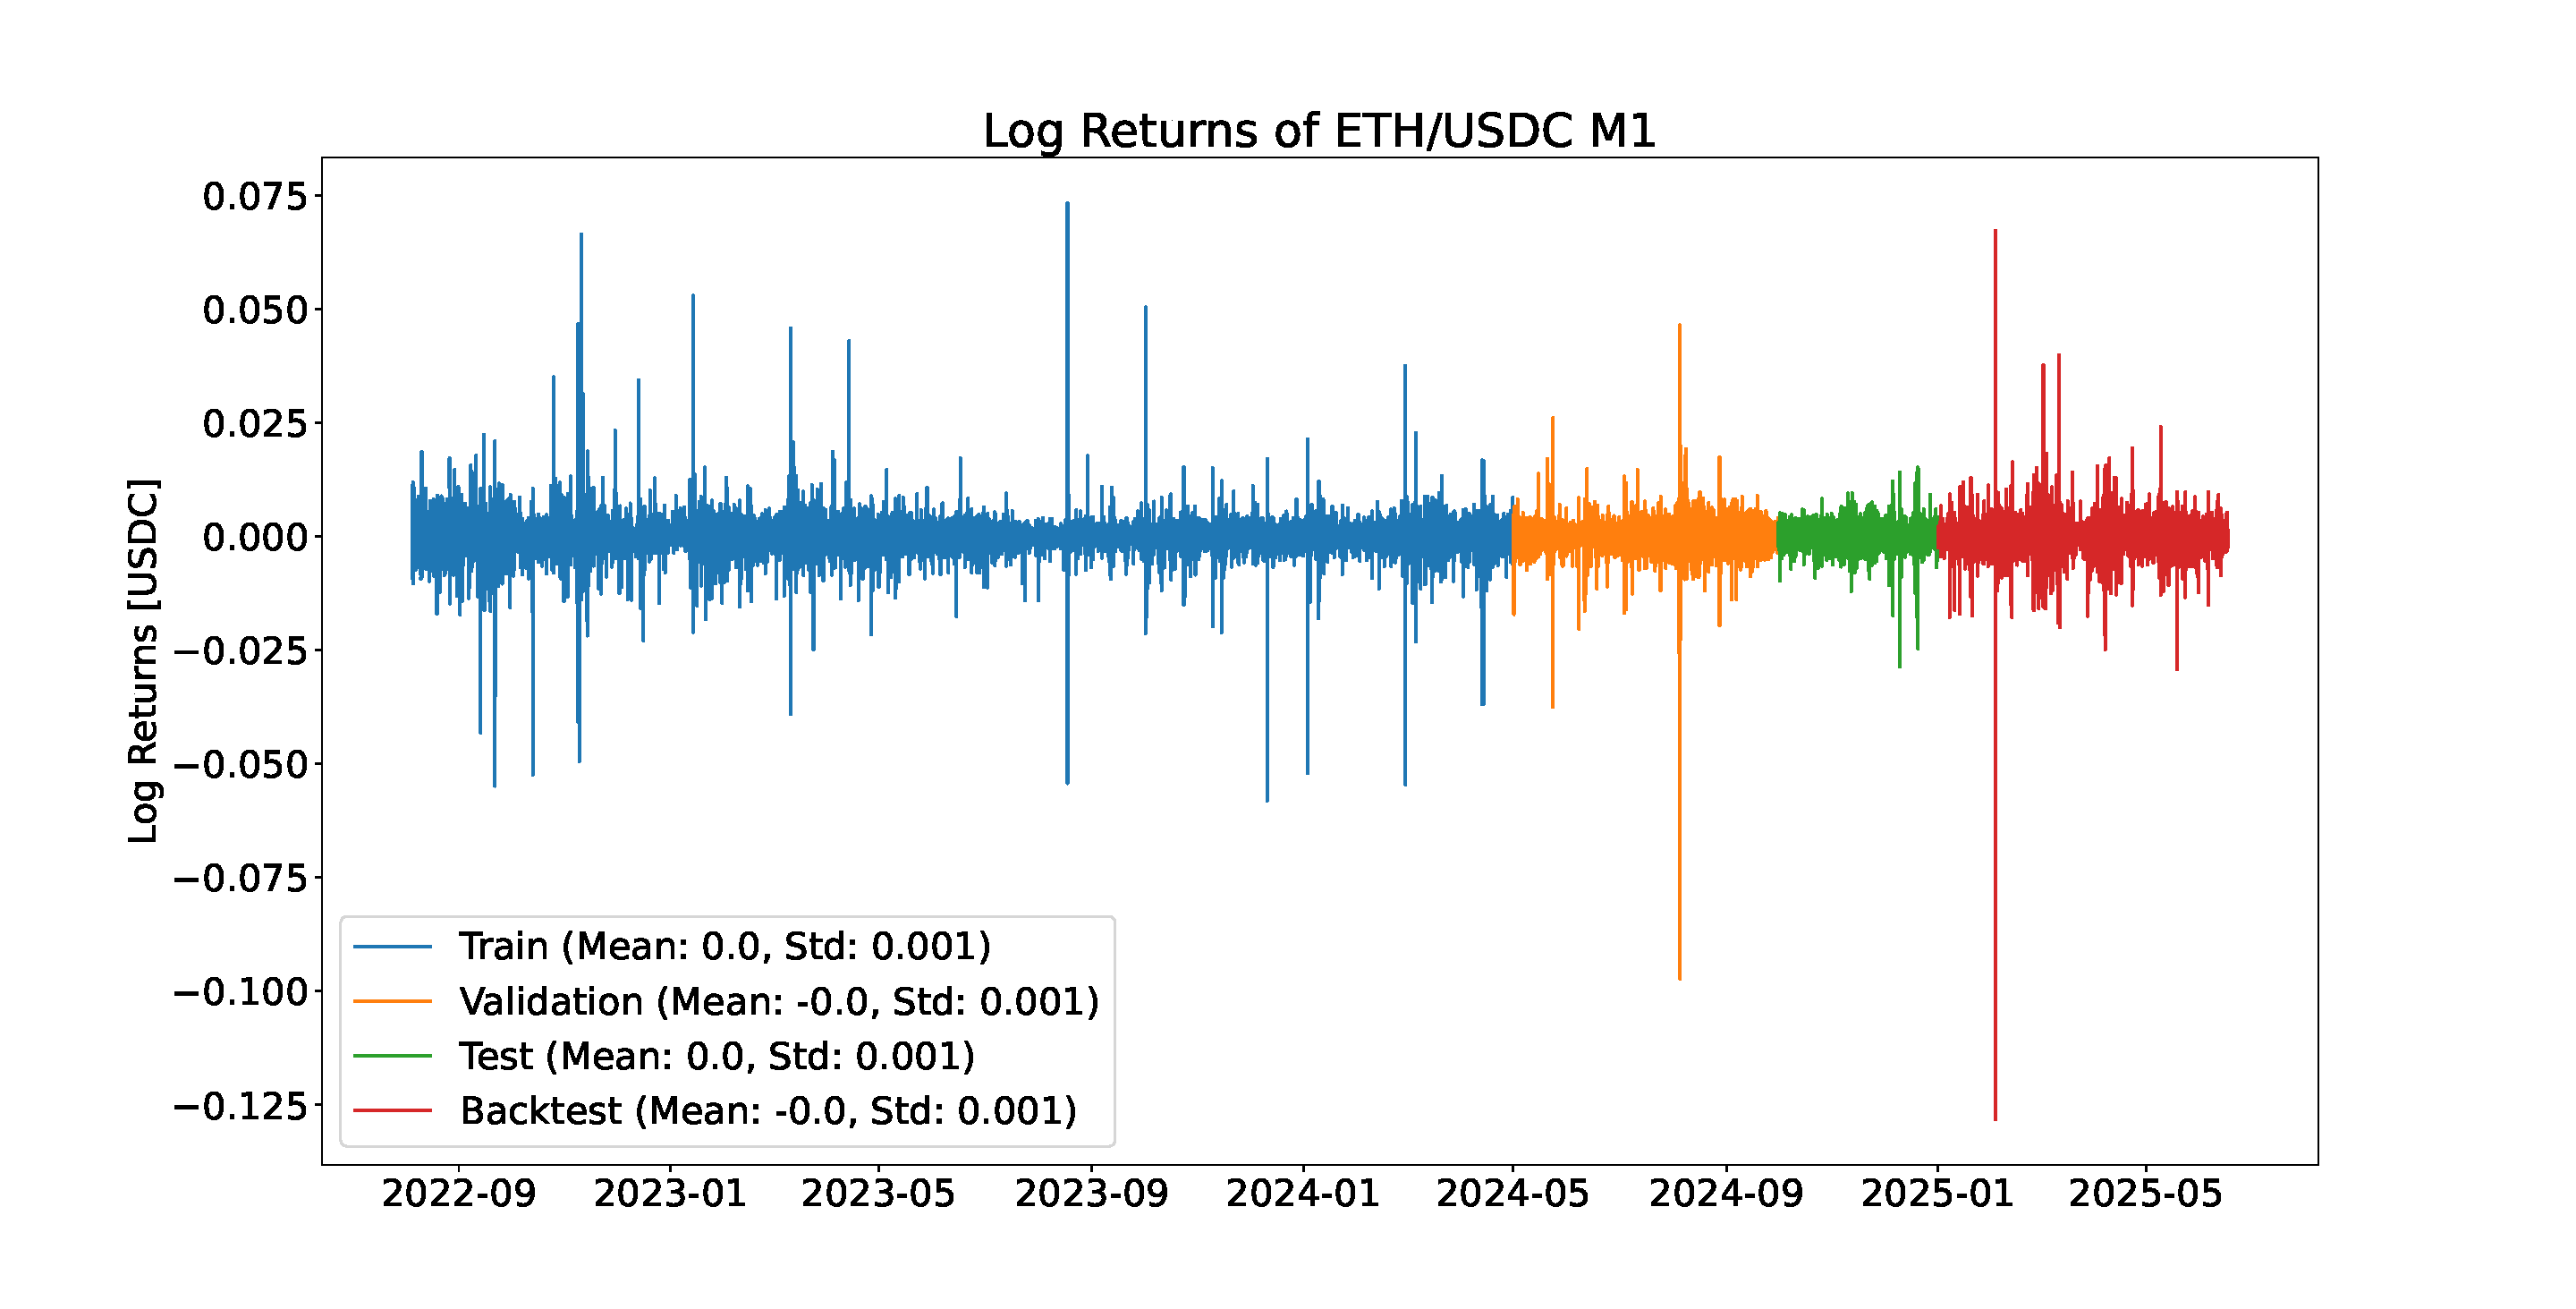
\includegraphics[width=\textwidth]{images/eda/log_returns_ethusdc}
    \caption{Log Returns of ETH in USDC}
    \label{fig:eth-log-data}
\end{figure}

\noindent
If an exact price is to be restored from the logarithmic returns, this can be done with the previous price using the following formula, which can be derived by transformation:

\[
    Price_t = Price_{t-1} \cdot e^{LogReturn_t}
\]

\noindent
If a series of logarithmic returns is present, any price in the series can also be calculated using the following formula, where $Price_{0}$ is the price at the start of the series and $t$ is the distance to the start of the series:

\[
    Price_t = Price_0 \cdot \prod_{i=0}^{t} e^{LogReturn_{i}} = Price_0 \cdot e^{\sum_{i=0}^{t} LogReturn_i}
\]

\noindent
The transformation is applied to the open, high, low, and close prices, and the original prices are replaced by the logarithmic returns, so that all subsequent actions are carried out using the logarithmic returns.

\subsection{Additional Features}
\label{chap:additional-features}

To provide the machine learning models with more context about the price, additional features from different categories were added to the transformed OHLCV data.

\subsubsection{Trend Following Indicators}

In financial analysis trend following indicators play an essential role while modeling and predicting future price movements.
This occurs because markets move in trends that are repeatedly interrupted by outliers.
This results in a zigzag movement that nevertheless moves in one direction.
Trend-following indicators can be used to filter out these outliers \cite{investopia-trend-indicators}.

The exponential moving average (EMA) is one type of trend following indicator.
It is a variation of the classic simple moving average (SMA), placing more emphasis on newer prices.
It is often used by traders in lengths of 10, 50, and 200 periods.

An important aspect of distinguishing between EMA and SMA is that many traders assume that new data better reflects the current trend, while others argue that giving more weight to recent prices can lead to distortion
\cite{investopia-ema}.

Since the aim of this paper is short-term predictions and the EMA reacts faster to price changes than the SMA, the EMA could provide more relevant context for the model.
The EMA was added in periods of 5, 10, 20, 30, 50, and 200 to the data.

Another trend following indicator is the moving average convergence/divergence \\(MACD) which does not only help to identify price trends, but also helps to measure the trend momentum.
It shows the relationship between two exponential moving averages.
To calculate the MACD line, an EMA(12) is subtracted from an EMA(26).
Additionally, a signal line is calculated as an EMA(9) of the MACD line \cite{investopia-macd}.


Although the MACD can signal possible reversals, it is also known for generating a significant number of false positives.
This tends to occur particularly in sideways or ranging markets, where price movements lack strong momentum or clear directional trends.
In such environments, the MACD lines frequently cross without a meaningful shift in market sentiment, leading traders to act on misleading signals.
Consequently, relying solely on MACD in these conditions can result in wrong entries or exits \cite{investopia-macd}.
To mitigate this, many traders combine MACD with additional indicators, such as support and resistance levels or trend confirmation tools, to improve decision-making and reduce noise.

Despite its susceptibility to false signals in sideways markets, the MACD can still be useful as a feature in a machine learning model.
This is because the indicator provides valuable information about momentum and potential trend changes, especially during periods of clear price movements.
In a machine learning context, the MACD is not considered in isolation but processed in combination with many other features.
This allows the model to learn under which market conditions the MACD is more reliable and when it should be ignored.
The nonlinear relationships and interactions with other features allow the model to identify context-dependent patterns from the MACD signals, which can be useful for predicting price movements.


\subsubsection{Volatility Indicators}

To measure volatility, there are other indicators and techniques in addition to those described in \autoref{chap:market-regime-categories}.

One such indicator is the average true range (ATR) which decomposes the entire range of an asset price over a period.
It is calculated by determining the so-called true range (TR) for each candlestick.
It is defined as the maximum of:

\begin{enumerate}
    \item Current high minus current low.
    \item Absolute distance from the previous closing price upwards.
    \item Absolute distance from the previous closing price downwards.
\end{enumerate}

\noindent
The ATR is then the moving average of these TR values, usually over 14 periods.

The ATR has two main limitations.
The first is that an ATR value must always be compared to previous ATR values, because one single value is not enough to tell if a trend is going to reverse.
The second limitation is that the ATR does not provide any information about the direction of the price \cite{investopia-atr}.
The ATR was added to the data with periods of 5, 7, 10, 14, and 18.

Another volatility indicator is Bollinger Bands, which consist of three lines.
The middle line is a SMA of the closing prices.
The lower line is calculated by subtracting a certain number of price standard deviations from the middle line, while the upper line is calculated by adding a certain number of price standard deviations to the middle line.
Usually, this number is two standard deviations \cite{investopia-bb}.

The higher the volatility of the market in the recent closing prices, the wider the band become.
If the price of the market rises near the upper band, traders see the market as overbought.
Similarly, if the market falls near the lower band, the market could be oversold.
This allows generating possible entry and exit signals \cite{investopia-bb}.
The three lines were added to the data using 15, 20, and 25 period SMAs with double price standard deviation.

\subsubsection{Momentum Indicators}

Momentum measures the strength and direction of a price movement over a certain period of time.
Momentum indicators are useful because they provide insights into the strength of trending prices and can therefore indicate possible trend reversals \cite{investopia-momentum}.

A common momentum indicator is the relative strength index (RSI).
It measures the speed and magnitude of price movements by comparing the average gains and losses over a specified period and can be used to detect overbought and oversold conditions.
The RSI ranges from 0 to 100.
Typically, an RSI above 70 indicates an overbought market, while an RSI below 30 indicates an oversold market.
The default RSI period commonly used for comparing average gains and losses is 14 \cite{investopia-rsi}.
The RSI was added to the data with periods of 7, 14, and 20.

To depict relative trend strength more precisely, a custom momentum indicator was constructed that compares the logarithmic returns of two different time frames, by subtracting the logarithmic returns of the two time frames.
This feature allows the model to distinguish phases of accelerating price movements from stable or declining trends.
The use of logarithmic returns simultaneously achieves scale independence and improved comparability, which is particularly advantageous for modeling financial market-related time series.
This indicator was added for time frames M2, M3, M6, M9, and M12.

\subsubsection{Price Transformation Indicators}

Apart from the mentioned indicators, shifted logarithmic returns for the recent six minutes have been added to provide additional context about the recent price movements in a compact form.
This can help the models to recognize trend reversals, volatility changes or short-term patterns.

Lastly, the logarithmic returns of other time frames (M2, M3, M6, M9, and M12) have been added to the data, providing a more stable trend context that helps correctly classify short-term price movements.
This creates a balanced feature set that takes into account both rapid reactions and long-term patterns.

\subsection{Further Transformations}

Due to the previous steps, the data contains 56 features (transformed OHLCV price data and additional indicators).
Two further transformations are then performed on the features.
This includes scaling and dimensionality reduction.
It is important to note that before these steps, the data is clustered into the respective regimes using the algorithm described in \autoref{chap:market-regimes}, and both scaling and dimensionality reduction are performed separately for each regime.
This brings advantages in both steps.

When scaling, the value range of the scaler can be better utilized.
This is evident, for example, with volatility indicators such as the ATR.
This indicator generates higher values in volatile phases than in less volatile ones.
If the scaler is fitted to the entire data and then a differentiation between market regimes is made, the entire value range of the scaler cannot be utilized in the respective regimes.
However, once the differentiation into regimes is made, the entire value range is utilized for each regime.

Dimensionality reduction also offers an advantage.
Here, different features may be more dominant than others in different regimes.
This allows examining which features are most important for each regime individually, preventing dilution.

\subsubsection{Scaling the Data}

Scaling data is an important step in exploratory data analysis.
This is because, on the one hand, machine learning models perform better with scaled data \cite{data-scaling} and, on the other hand, principal component analysis (\autoref{chap:pca}) is sensitive to unscaled data \cite{pca-scaling}.

The use of the scikit-learn \texttt{MinMaxScaler} \cite{min-max}, which scales data in a fixed range of $[0; 1]$ is useful and widely adopted.
Neural networks, especially those with activation functions such as ReLU, which are introduced in \autoref{chap:nn}, benefit greatly from inputs with a uniform range of values.
The scaling stabilizes the gradient flow, shortens training time and reduces vanishing gradients \cite{min-max-benefits}.

For these reasons, all features were scaled with the \texttt{MinMaxScaler} and are used exclusively in scaled form in all steps related to machine learning.

\subsubsection{Principal Component Analysis}
\label{chap:pca}

The principal component analysis (PCA) is a process for dimensional reduction, by linearly transforming high dimensional datasets into a small number of uncorrelated principal components  (directions of the new coordinate system).
During the transformation, it can be specified how much variance in the data is retained.
After a transformation using PCA, it is ensured that at least the specified variance is retained \cite{wikipedia-pca}.

Especially when processing numerous technical indicators or derived features in financial data, the high dimensionality can become problematic - a phenomenon known as the curse of dimensionality.
This term describes the increasing challenges in modeling as the number of dimensions or features increases.
Data points become increasingly sparsely distributed, computational costs increase, and many models lose their ability to generalize.
Applying PCA allows redundant or correlated information to be condensed, making the model more robust, faster, and easier to interpret.
At the same time, the risk of overfitting is reduced because the model focuses on the most important structures in the dataset \cite{wikipedia-curse-od-dimensionality}.

\autoref{fig:explained-variance} shows the cumulative explained variance for the 56 added features in \autoref{chap:additional-features} for each quantile market regime.
It shows that the cumulative variance increases rapidly at the beginning.
In this case, the reduction of the projection to just 3 to 6 principal components already explains at least 80\% of the variance.
This means that the majority of the statistically relevant structures in the dataset are retained, even though the number of features has been massively reduced.
Even if 20\% of the variance is lost, the benefit outweighs this: The remaining principal components capture the statistical essence of the original feature space in a significantly more compact and robust form, which is particularly well-suited for machine learning.


\begin{figure}[H]
    \centering
    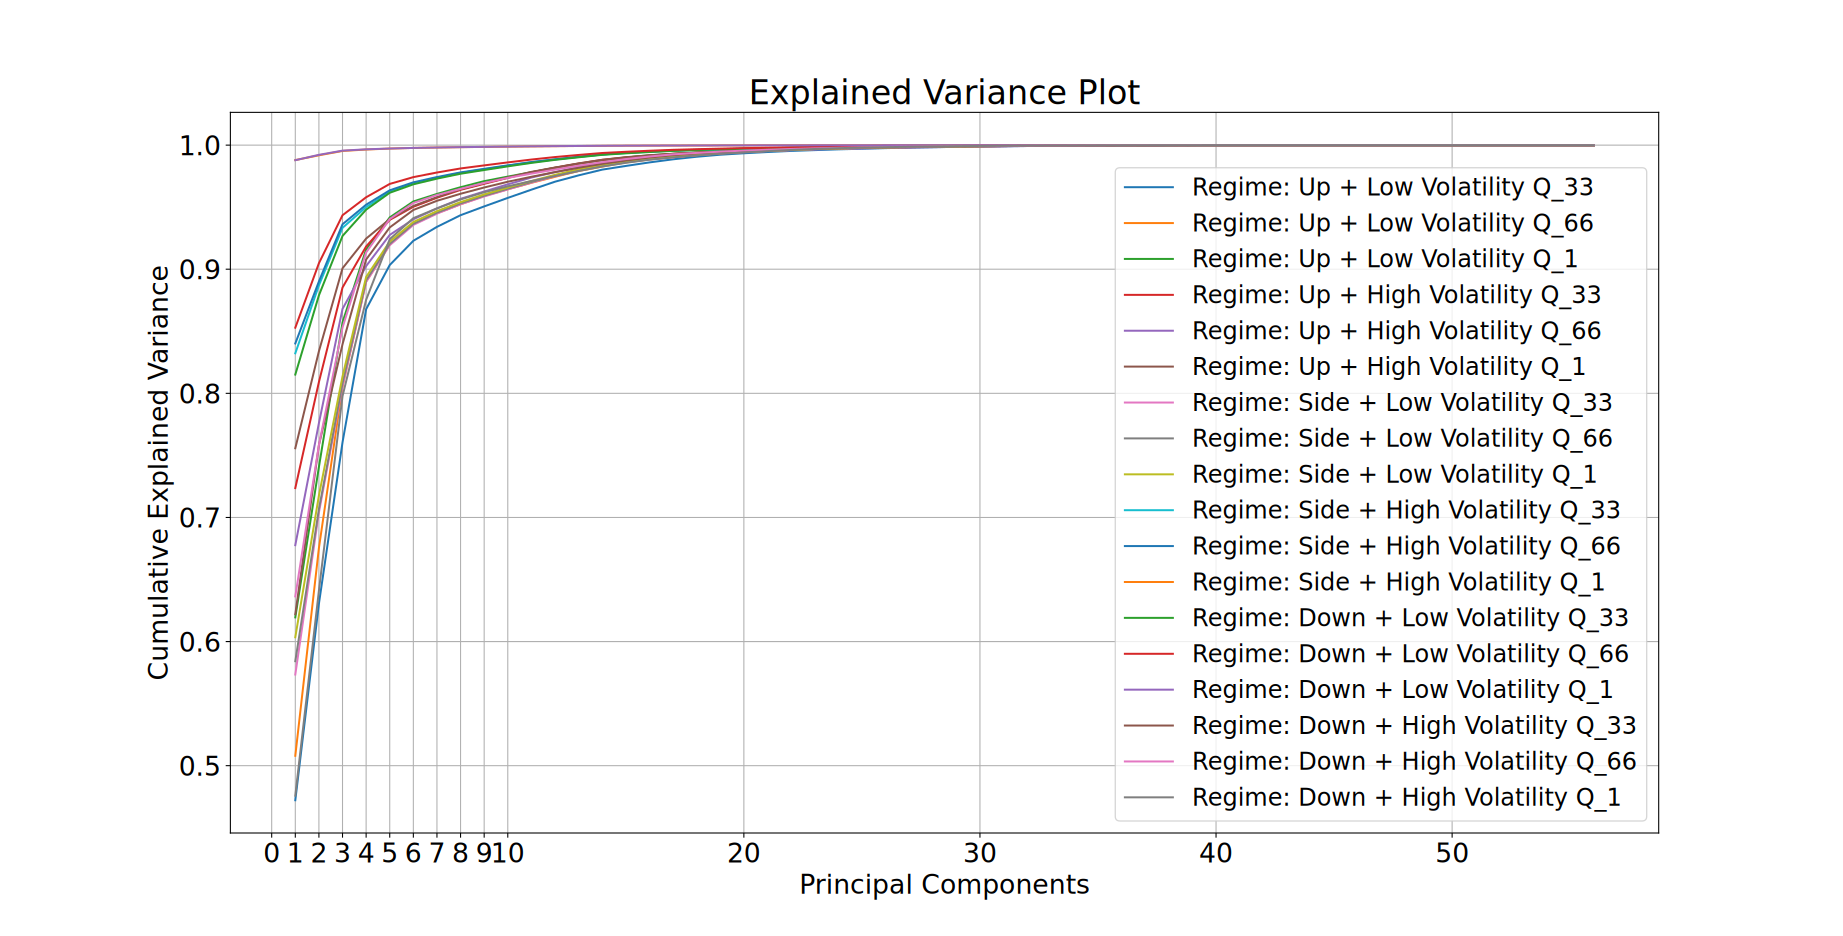
\includegraphics[width=\textwidth]{images/eda/explained_variance}
    \caption{Cumulative Explained Variance}
    \label{fig:explained-variance}
\end{figure}
